%% Report on the S3-3HDM fermion sector.
%% Companion: derivations_02.tex (the derivation ledger, auto-generated by the notebook).
%% Source: research/thdm_s3/02_s3_fermion_sector.ipynb
\documentclass[11pt,a4paper]{article}
\usepackage[T1]{fontenc}
\usepackage[utf8]{inputenc}
\usepackage{amsmath,amssymb}
\usepackage{graphicx}
\usepackage{booktabs}
\usepackage[margin=2.4cm]{geometry}
\usepackage[colorlinks=true,linkcolor=blue,citecolor=blue,urlcolor=blue]{hyperref}
\setlength{\parindent}{0pt}
\setlength{\parskip}{0.6em}

\title{The $S_3$-symmetric 3HDM fermion sector:\\
three corrections to the LFVHD draft, and why exact $S_3$\\
forces $V_{us}=0$}
\author{M. Zeleny-Mora\\[2pt]
\small Instituto de Física, Universidad Nacional Autónoma de México}
\date{\today}

\begin{document}
\maketitle

\begin{abstract}
\noindent
I have rebuilt the fermion sector of our LFV draft \cite{LFVHD} from the Lagrangian, using
the draft's own $S_3$ assignment, and checked every derivation in it. The charged-lepton
Yukawa sector is invariant and complete. Three defects turned up, and all three are now
corrected in \texttt{LFVHD\_3HDMS3.tex}. The one with consequences is that $\mu_5=\mu_4$ is an
\emph{assumption}, not a result: it follows from matching masses to eigenvalues rather than
singular values. The draft does not treat quarks, so I added them, and this gives the
substantive result. With exact $S_3$ the CKM matrix is forced to be a pure $2$--$3$
rotation, $V_{us}=V_{ub}=V_{cd}=V_{td}=0$, for \emph{any} Yukawa couplings. The cause is the
same residual $\mathbb Z_2$ that the vacuum alignment preserves. Soft $S_3$ breaking lifts
it: a bounded fit then reproduces the six quark masses and $|V_{us}|$, $|V_{cb}|$,
$|V_{ub}|$ simultaneously. The CP phase stays out of reach, because these Yukawas are real.
\end{abstract}

\section{Summary}

Everything below comes from \texttt{research/thdm\_s3/02\_s3\_fermion\_sector.ipynb}. It
takes the $S_3$ assignment, the Yukawa Lagrangian and the diagonalisation strategy from
\cite{LFVHD}. Everything else is derived with \texttt{feynlag}, including every check of
the draft.

\begin{enumerate}\itemsep2pt
\item \textbf{The draft and our code use different $S_3$ doublet bases}, related by a reflection at
$\pi/6$. For the Yukawas the coupling dictionary comes out as the identity. This contrasts
with the scalar potential, where the same analysis flips the sign of $\lambda_4$
(\S\ref{sec:basis}).
\item \textbf{The lepton Yukawa sector is invariant and complete}: five structures, all
gauge- and $S_3$-invariant, and an independent enumeration finds exactly five
(\S\ref{sec:leptons}).
\item \textbf{Three defects in the draft}, all corrected in the \texttt{.tex}. One needs
further wording in the draft: $\mu_5=\mu_4$ should be stated as an assumption
(\S\ref{sec:defects}).
\item \textbf{Exact $S_3$ forces $V_{us}=0$} (\S\ref{sec:ckm}), which is the main result.
\item \textbf{Soft $S_3$ breaking switches the Cabibbo angle on}, at no cost to the scalar
constraints (\S\ref{sec:soft}).
\end{enumerate}

\section{The two bases}
\label{sec:basis}

The draft's doublet generators are $a=R(-2\pi/3)$ and $b$, a reflection about $30^\circ$.
\texttt{feynlag}'s are $\rho(a)=R(2\pi/3)$ and $\rho(b)=\mathrm{diag}(1,-1)$. The two are
conjugate by a unique $O(2)$ map, the reflection at $\pi/6$:
\[
O=\begin{pmatrix}\cos\frac\pi6&\sin\frac\pi6\\ \sin\frac\pi6&-\cos\frac\pi6\end{pmatrix},
\qquad O^{-1}\rho(g)\,O=\rho_{\rm draft}(g),\qquad \det O=-1 .
\]
This is why the draft's alignment reads $v_1=\sqrt3\,v_2$ while ours reads
$v_2=\sqrt3\,v_1$. Of the five Yukawa structures, four are dot products of two doublets and
do not depend on the basis. Only the triple-doublet structure ($Y_2$) changes. Each form is
invariant in its own basis and fails in the other. Under $O$ the draft's form maps to ours
with coefficient $+1$, so the coupling dictionary is the identity.

The vacuum needs one remark. The map sends our aligned vacuum $(v_1,\sqrt3 v_1)$ to
$(\sqrt3 v_1,-v_1)$, which is the draft's $|v_1/v_2|=\sqrt3$ but with $v_2<0$. The sign
carries no physics. The mass matrix obeys $M(-r)=P\,M(r)\,P$ with
$P=\mathrm{diag}(-1,1,1)$, which is a sign flip of the first-generation fields, so masses and $|$mixings$|$ are
unchanged.

\section{The lepton sector is invariant and complete}
\label{sec:leptons}

With $(L_1,L_2)$, $(e_{1R},e_{2R})$ as doublets and $L_S$, $e_{SR}$ as singlets
\cite{LFVHD}, all five structures $Y_k^\ell T_k$ pass $SU(2)_L$, $U(1)_Y$ and $S_3$
invariance, and the Lagrangian with its h.c.\ is hermitian. The draft's literal $T_2$ fails
$S_3$, as it must, because it is written in the other basis. \texttt{feynlag}'s own
enumeration of $S_3$- and gauge-invariant Yukawa operators, run independently of the draft,
returns exactly five. The charged-lepton Yukawa sector of \cite{LFVHD} is complete.

\section{Three defects in the draft, all corrected}
\label{sec:defects}

\paragraph{1. The $\mu\leftrightarrow Y$ dictionary was a factor $\sqrt2$ too large.}
The draft writes an explicit $1/\sqrt2$ on the Yukawa structures and also expands
$\langle H_i^0\rangle=v_i/\sqrt2$. Composing the two gives, for example,
$\mu_1^\ell=Y_1^\ell v_3/2$, where the draft printed $v_3Y_1^\ell/\sqrt2$. All five printed
$\mu_k$ exceed the Lagrangian's by exactly $\sqrt2$, which makes it a convention slip
($\langle H^0\rangle=v$ instead of $v/\sqrt2$) and not a typo. Nothing physical depends on
it, since the $\mu$'s are eliminated in favour of the masses. It matters only if one quotes
the Yukawa couplings themselves.

\paragraph{2. Eigenvalues versus singular values; $\mu_5=\mu_4$ is an assumption.}
After $O_{12}$ the residual block is
$A=\begin{pmatrix}\rho&2\mu_5\\2\mu_4&\mu_3\end{pmatrix}$ with $\rho=\mu_1+2\mu_2$. The
physical masses are its \emph{singular} values. From $\sigma_1^2+\sigma_2^2=\mathrm{tr}(A^{\mathsf T}A)$ and
$\sigma_1\sigma_2=\det A$,
\[
(\sigma_1-\sigma_2)^2=(\rho-\mu_3)^2+4(\mu_4+\mu_5)^2 ,
\]
while the draft printed $+16\mu_4\mu_5$. That is $(\mathrm{tr}A)^2-4\det A$, the gap
between the \emph{eigenvalues}. The two agree only when $\mu_4=\mu_5$. More important,
$\mu_5=\mu_4$ is not forced by the masses. It is equivalent to imposing the trace relation
$m_\mu+m_\tau=\mathrm{tr}A$, i.e.\ to the ansatz $O_L=O_R$. The notebook exhibits a
$\mu_4\neq\mu_5$ point with valid masses as singular values (singular values
$2.539,\ 0.291$; eigenvalues $2.232,\ -0.332$; $\mathrm{tr}A=1.9$). The corrected
\texttt{.tex} fixes the formula, but it still uses the trace relation, so \textbf{the draft
should state $\mu_5=\mu_4$ as an assumption}. This is the one wording change still open.

\paragraph{3. A coefficient slip.}
In the $\mu_5=0$, $\mu_3=m_\mu$ case,
$\mathrm{tr}(A^{\mathsf T}A)=m_\mu^2+m_\tau^2+4\mu_4^2$, where the draft printed $2\mu_4^2$.
The conclusion $\mu_4=0$ is unaffected.

\paragraph{What checks out.}
Everything else in the draft's fermion sector agrees with an independent derivation:
\begin{itemize}\itemsep1pt
\item $R_S=R_AR_H$ holds identically;
\item $O_{12}$ block-diagonalises the $1$--$2$ sector for \emph{any} vacuum ratio, and at the
alignment the first generation decouples with $m_e=\mu_1-2\mu_2$;
\item $\tan2\theta_\ell=-4\mu_4/(m_\mu+m_\tau-2\mu_3)$ and the $p_{1,2}$ closed forms agree;
\item $Q_1(A)=\mathrm{diag}(m_e,m_\mu,m_\tau)/v$.
\end{itemize}
The last is an identity, $Q_1(A)=O^{\mathsf T}MO/v$ for any orthogonal $O$. It pins the vacuum
geometry rather than the rotation, so the $G_k$ decomposition of $M_\ell$ is checked
separately.

\section{Main result: exact $S_3$ forces $V_{us}=0$}
\label{sec:ckm}

The quark sector has ten Yukawa structures: five down-type through $H$ and five up-type
through $\tilde H$. All ten are $S_3$-, $SU(2)_L$-, $U(1)_Y$- and $SU(3)_c$-invariant.
Because the $S_3$ matrices are real, $\tilde H$ is the same $S_3$ doublet as $H$, so
\textbf{$M_u$ and $M_d$ have identical structure}. Only the couplings differ.

The $1$--$2$ block-diagonalising rotation satisfies
\[
\tan2\psi=-r,\qquad r\equiv v_1/v_2 \ \ \text{(draft basis)},
\]
and so depends on the \emph{vacuum alone}, never on the Yukawas. The same $O_{12}$
therefore acts on the up, down and charged-lepton sectors. The first generation decouples
from the other two iff its eigenvector is orthogonal to $(r,1)$, which reduces to
\[
r\,\big(2-\sqrt{r^2+1}\big)=0\qquad\Longleftrightarrow\qquad |r|=\sqrt3\ \ (\text{or }r=0),
\]
exactly the vacuum that preserves the residual $\mathbb Z_2$. With exact $S_3$ the
tadpoles force that vacuum. So
\[
V_{\rm CKM}=O_u^{\mathsf T}O_d=O_{23}(\theta_u)^{\mathsf T}O_{12}^{\mathsf T}O_{12}O_{23}(\theta_d)
=O_{23}(\theta_d-\theta_u),
\]
a pure $2$--$3$ rotation, with $V_{us}=V_{ub}=V_{cd}=V_{td}=0$ for arbitrary Yukawas. This
is checked numerically to machine precision, and the root $\sqrt3$ is isolated: the
decoupling entry is non-zero at $r=2,\ 3/2,\ \sqrt5,\ 1/2$. The form $O_{12}O_{23}$ uses
the $\mu_5=\mu_4$ ansatz, but $V_{us}=0$ does not: at $|r|=\sqrt3$ the first generation
decouples from both rows and columns either way.

The mechanism is the one of Das, Dey and Pal \cite{DasDeyPal16}: an unbroken $\mathbb Z_2$
gives an approximately block-diagonal CKM matrix. \textbf{The block, however, is
different.} There the Cabibbo block stays free, and soft breaking generates only the small
elements. With the draft's assignment the block is $2$--$3$, so $V_{us}$ itself vanishes,
against a measured $|V_{us}|=0.2243$ \cite{PDG}. The exact-$S_3$ quark sector is excluded.

\section{Soft $S_3$ breaking switches the Cabibbo angle on}
\label{sec:soft}

Soft breaking means $S_3$-violating terms of dimension below four, which here are
quadratics only. In the CP-conserving case the hermitian quadratics $\mu_{ij}^2H_i^\dagger
H_j$ have six real parameters, two of them $S_3$-invariant, leaving four soft ones: the
$\mathbf2$ pair $(x_{11}-x_{22},\,x_{12}+x_{21})$ and $(H_S^\dagger H_{1,2}+\text{h.c.})$.
Two consequences:
\begin{itemize}\itemsep1pt
\item \textbf{no quartic is touched}, so every boundedness and unitarity result of the
scalar-sector report carries over unchanged;
\item \textbf{the vacuum is freed}: the tadpole system stops being over-constrained, $r$ is
no longer pinned to $\sqrt3$, and the $\mathbb Z_2$ breaks.
\end{itemize}

\begin{figure}[h]
\centering
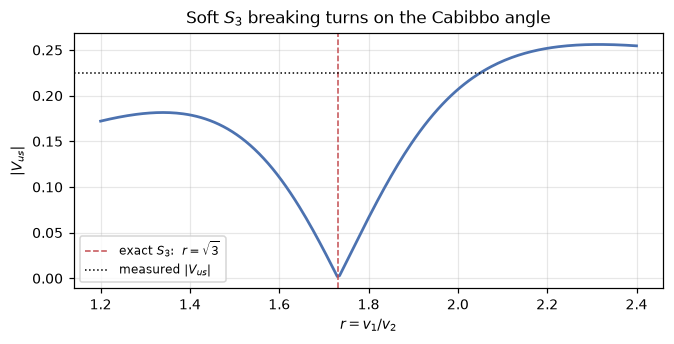
\includegraphics[width=0.78\textwidth]{figures/fermion_vus_vs_r.png}
\caption{$|V_{us}|$ against the vacuum ratio $r$ at fixed Yukawas. It vanishes exactly at
the exact-$S_3$ vacuum ($|V_{us}|=4.6\times10^{-17}$ at $r=\sqrt3$) and grows linearly away
from it: the ratio of its values at $r=\sqrt3+0.05$ and $\sqrt3+0.025$ is $1.999$.}
\label{fig:vus}
\end{figure}

To show that the mechanism reaches the observed values, I fitted the eight Yukawa
parameters $(\mu_1,\ldots,\mu_4)_{u,d}$ plus $r$ to the six quark masses and three CKM
magnitudes \cite{PDG}. The fit converges (cost $2.8\times10^{-26}$) at
\[
r=1.3487\quad(\text{exact }S_3:\ \sqrt3=1.7321),\qquad r-\sqrt3=-0.383 ,
\]
reproducing all nine targets:
\begin{center}
\begin{tabular}{lccc}
\toprule
 & $|V_{us}|$ & $|V_{cb}|$ & $|V_{ub}|$\\
\midrule
fit & $0.22430$ & $0.04110$ & $0.00382$\\
target \cite{PDG} & $0.2243$ & $0.0411$ & $0.00382$\\
\bottomrule
\end{tabular}
\end{center}
together with the six masses,
\[
(m_u,m_c,m_t)=(0.00216,\ 1.27,\ 172.69)~\text{GeV},\qquad
(m_d,m_s,m_b)=(0.00467,\ 0.0934,\ 4.18)~\text{GeV}.
\]
The fit is stored in \texttt{results/quark\_soft\_fit.json}.

Two caveats govern how to read this.
\begin{itemize}\itemsep1pt
\item \textbf{$r$ is an existence proof, not a prediction.} Nine parameters against nine
targets is an exactly determined system. Different restarts land on different exact
solutions at different $r$, and so does a different numpy/scipy version. What the fit
establishes is that the two-stage structure does \emph{not} prevent the three magnitudes
from being matched simultaneously.
\item \textbf{The CP phase is structurally out of reach.} The Yukawas are real, so the CKM
matrix is real and the Jarlskog invariant vanishes identically.
\end{itemize}

Where this vacuum sits in the soft-broken \emph{scalar} scan is the subject of the
companion report on the soft-broken vacuum. The fit's $|r|=1.349$ corresponds to
$\varphi=53.4^\circ$ inside the scanned domain, a well-populated region.

\section{The neutrinos the draft declares but does not use}

\cite{LFVHD} assigns $(\nu_{1R},\nu_{2R})$ to a $\mathbf2$ and $\nu_{SR}$ to a $\mathbf1$, and
then writes no neutrino Yukawa or mass term. These fields are not inert. \texttt{feynlag}
enumerates five further $S_3$- and gauge-invariant Dirac structures through $\tilde H$, the
same pattern as the charged leptons. Majorana $\nu_R$ masses would come on top of these;
they were not enumerated. The charged-lepton sector is complete; the neutrino sector is
simply absent.

\section{Open questions, and what would help}

\begin{enumerate}\itemsep4pt
\item \textbf{State $\mu_5=\mu_4$ as an assumption in the draft} (\S\ref{sec:defects}). It is
the $O_L=O_R$ ansatz. The masses alone do not force it.
\item \textbf{A complex-Yukawa extension.} The soft-broken fit matches the three CKM
magnitudes, but $J=0$ identically. Whether complex Yukawas can also reproduce
$\delta_{\rm CP}$ is open.
\item \textbf{The neutrino sector}: the Dirac Yukawas through $\tilde H$ and the Majorana
$\nu_R$ masses. \texttt{feynlag} has the seesaw machinery, so this is a matter of doing it.
\item \textbf{Does the quark structure belong in the LFV paper?} The CKM obstruction and the
LFV structure come from the same $O_{12}$, and $\mathcal B(h\to\tau e)=0$ exactly in the
decays report is the leptonic face of $V_{us}=0$. My instinct is that a short section is
worth it. Your call.
\end{enumerate}

\appendix
\section{The derivation ledger}

The full typeset version is the companion document \texttt{derivations\_02.tex}; in
summary:

\begin{center}
\begin{tabular}{p{0.30\textwidth}p{0.13\textwidth}p{0.47\textwidth}}
\toprule
claim & status & independent checks\\
\midrule
$\mu_k=Y_kv/\sqrt2$, and the draft's uniform factor $\sqrt2$ & derived &
read off the extracted mass matrix; all five ratios equal; rebuilding with the draft's own
prefactors reproduces its printed values exactly\\
\addlinespace
$(\sigma_1-\sigma_2)^2=(\rho-\mu_3)^2+4(\mu_4+\mu_5)^2$ & derived &
built from $\mathrm{tr}(A^{\mathsf T}A)$ and $\det A$; symmetric under $\mu_4\leftrightarrow\mu_5$; the
printed form is shown to be the eigenvalue gap\\
\addlinespace
First-generation decoupling iff $|r|=\sqrt3$, hence $V_{us}=0$ & derived &
eigenvector taken from \texttt{eigenvects()}, not written down; isolated root; numeric
$V_{\rm CKM}$ at arbitrary Yukawas\\
\addlinespace
The $S_3$ lepton assignment and its five structures & \textbf{imported} \cite{LFVHD} &
all five invariant; an independent enumeration finds exactly five\\
\bottomrule
\end{tabular}
\end{center}

\begin{thebibliography}{9}

\bibitem{LFVHD} M.~Zeleny-Mora, M.~Mondragón and T.~A.~Valencia-Pérez,
\emph{Exploring LFV Higgs decays in the Three Higgs Doublet Model}, draft
(\texttt{paper\_lfvhd/LFVHD\_3HDMS3.tex}).

\bibitem{DasDeyPal16} D.~Das, U.~K.~Dey and P.~B.~Pal,
\emph{$S_3$ symmetry and the quark mixing matrix},
Phys.\ Lett.\ B \textbf{753}, 315 (2016),
\href{https://arxiv.org/abs/1507.06509}{arXiv:1507.06509},
\href{https://doi.org/10.1016/j.physletb.2015.12.038}{doi:10.1016/j.physletb.2015.12.038}.

\bibitem{PDG} S.~Navas \emph{et al.} (Particle Data Group),
\emph{Review of Particle Physics}, Phys.\ Rev.\ D \textbf{110}, 030001 (2024),
\href{https://doi.org/10.1103/PhysRevD.110.030001}{doi:10.1103/PhysRevD.110.030001}.

\end{thebibliography}

\end{document}
